% !TEX root = ../main.tex

\chapter{Template}

Write your template examples here.

\begin{figure}[htbp]
	\centering
	
\includegraphics[width=0.8\textwidth]{figures/flower.png}
	\caption{Description of the flower.}
	\label{fig:flower}
\end{figure}



We have some text before the inserted PDF ...

% --- Importing PDF files
% Imported a specific page of a pdf file
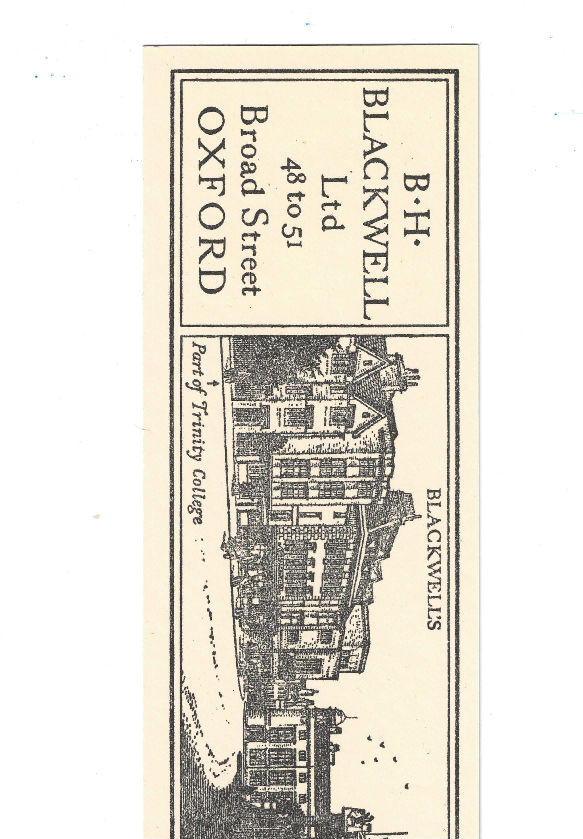
\includepdf[pages=1]{figures/example1v.pdf}

% --- All pages:
% \includepdf[pages=-]{figures/report_appendix.pdf}

% --- Specific pages with a fitting mode:
% \includepdf[pages={2,4-6}, fitpaper=true]{figures/document.pdf}

We have some text after the inserted PDF ...

\section{Example Table}

Table~\ref{tab:example} shows a simple comparison.

\begin{table}[htbp]
	\centering
	\caption{Comparison of example values.}
	\label{tab:example}
	\begin{tabular}{lcc}
		\toprule
		\textbf{Category} & \textbf{Value A} & \textbf{Value B} \\
		\midrule
		Alpha  & 12.4 & 8.1  \\
		Beta   & 9.7  & 14.3 \\
		Gamma  & 15.2 & 11.6 \\
		\bottomrule
	\end{tabular}
\end{table}

\section{Example Citation}

Bias in machine learning models often originates from unbalanced training data
rather than flawed algorithms \citep{smith2021}. As Smith and Jones (2021)
demonstrate \citep{smith2021}, this distinction has significant implications
for how practitioners approach model auditing.

\Gls{ai} is one of the most disruptive technologies.


\section{Example Lists}

\subsection{Bulleted List}

An unordered list is useful when items have no inherent sequence:

\begin{itemize}
	\item First point of consideration.
	\item Second point, independent of the first.
	\item Third point, with a nested sub-list:
	\begin{itemize}
		\item Sub-point A.
		\item Sub-point B.
	\end{itemize}
\end{itemize}

\subsection{Numbered List}

An ordered list is useful when sequence or ranking matters:

\begin{enumerate}
	\item Initial step of the process.
	\item Subsequent step, dependent on the first.
	\item Final step, concluding the sequence.
\end{enumerate}

\subsection{Description List}

A description list pairs a term with its explanation — useful for glossaries or defining terms:

\begin{description}
	\item[Bias] Systematic error introduced into a model due to unrepresentative training data.
	\item[Variance] Sensitivity of a model to small fluctuations in the training set.
	\item[Overfitting] A model that captures noise rather than underlying patterns.
\end{description}

% Referencing to online content on a website:
Recent evidence suggests pandemic-related isolation significantly increased
reported anxiety and depressive symptoms globally \citep{who2023}.

Model training in this project made use of the scikit-learn library
\citep{pedregosa2011}.

The Transformer architecture dispensed with recurrence entirely, relying
solely on attention mechanisms \citep{vaswani2017}. \\

\Gls{ml} models require large datasets.
% First occurrence renders as: "Machine Learning (ML) models require large datasets."
% Any subsequent \gls{ml} renders as just: "ML models require large datasets."

\Gls{api} adds the capability for subcomponents of an application to communicate with each other.

\Gls{ai} is one of the most disruptive technologies.

% -----------------------------------------------------------------
% LONG TABLES (crossing multiple pages)
% -----------------------------------------------------------------
% The standard `tabular` environment (used in the table examples
% above) does NOT break across pages — if content overflows, it
% either gets cut off or throws an overfull box warning.
%
% For tables that may span multiple pages (e.g. long datasets,
% detailed appendix listings), use `longtable` instead.
%
% REQUIRES: \RequirePackage{longtable} in mycls.cls (not yet added
% — add it if you use this).
%
% KEY DIFFERENCES FROM `tabular`:
%   - No \begin{table}...\end{table} wrapper — longtable is a
%     floating-like environment on its own; wrapping it in `table`
%     will break page-splitting.
%   - Caption and label go INSIDE the longtable environment, not
%     around it.
%   - \endhead marks header rows that repeat on every page.
%   - \endfoot / \endlastfoot let you define a footer that differs
%     on the final page (e.g. "continued on next page" vs a closing
%     \bottomrule).
%
% EXAMPLE:
%
% \begin{longtable}{ll}
	%     \caption{Overview of submitted files.} \label{tab:submitted-files} \\
	%     \toprule
	%     \textbf{File} & \textbf{Description} \\
	%     \midrule
	%     \endfirsthead
	%
	%     % Header repeated on subsequent pages:
	%     \multicolumn{2}{l}{\small\itshape (continued from previous page)} \\
	%     \toprule
	%     \textbf{File} & \textbf{Description} \\
	%     \midrule
	%     \endhead
	%
	%     % Footer on all pages except the last:
	%     \midrule
	%     \multicolumn{2}{r}{\small\itshape continued on next page} \\
	%     \endfoot
	%
	%     % Footer on the final page only:
	%     \bottomrule
	%     \endlastfoot
	%
	%     \texttt{main.pdf}       & Compiled report (this document). \\
	%     \texttt{main.tex}       & Main LaTeX source file.          \\
	%     % ... more rows ...
	%
	% \end{longtable}
%
% NOTE: longtable disables centering by default — wrap in
% \begin{center}...\end{center} if needed, or use the `ltcaption`
% package's alignment options.
% -----------------------------------------------------------------

\section{Example Long Table}

Table~\ref{tab:long-example} demonstrates a table spanning multiple pages,
with the header row repeating automatically on each page.

\begin{longtable}{ll}
	\longtablecaption{Example long table spanning multiple pages.}{tab:long-example}
	\toprule
	\textbf{Item} & \textbf{Value} \\
	\midrule
	\endfirsthead
	
	\multicolumn{2}{l}{\small\itshape (continued from previous page)} \\
	\toprule
	\textbf{Item} & \textbf{Value} \\
	\midrule
	\endhead
	
	\midrule
	\multicolumn{2}{r}{\small\itshape continued on next page} \\
	\endfoot
	
	\bottomrule
	\endlastfoot
	
	Entry 01 & 12.4 \\
	Entry 02 & 8.1  \\
	Entry 03 & 15.2 \\
	Entry 04 & 9.7  \\
	Entry 05 & 14.3 \\
	Entry 06 & 11.6 \\
	Entry 07 & 13.8 \\
	Entry 08 & 10.5 \\
	Entry 09 & 16.1 \\
	Entry 10 & 7.9  \\
	Entry 11 & 12.0 \\
	Entry 12 & 14.7 \\
	Entry 13 & 9.3  \\
	Entry 14 & 15.9 \\
	Entry 15 & 11.2 \\
	Entry 16 & 13.4 \\
	Entry 17 & 8.6  \\
	Entry 18 & 16.8 \\
	Entry 19 & 10.1 \\
	Entry 20 & 12.9 \\
	Entry 21 & 14.2 \\
	Entry 22 & 9.8  \\
	Entry 23 & 15.5 \\
	Entry 24 & 11.7 \\
	Entry 25 & 13.1 \\
	Entry 26 & 8.4  \\
	Entry 27 & 16.3 \\
	Entry 28 & 10.9 \\
	Entry 29 & 12.6 \\
	Entry 30 & 14.9 \\
Entry 01 & 12.4 \\
Entry 02 & 8.1  \\
Entry 03 & 15.2 \\
Entry 04 & 9.7  \\
Entry 05 & 14.3 \\
Entry 06 & 11.6 \\
Entry 07 & 13.8 \\
Entry 08 & 10.5 \\
Entry 09 & 16.1 \\
Entry 10 & 7.9  \\
Entry 11 & 12.0 \\
Entry 12 & 14.7 \\
Entry 13 & 9.3  \\
Entry 14 & 15.9 \\
Entry 15 & 11.2 \\
Entry 16 & 13.4 \\
Entry 17 & 8.6  \\
Entry 18 & 16.8 \\
Entry 19 & 10.1 \\
Entry 20 & 12.9 \\
Entry 21 & 14.2 \\
Entry 22 & 9.8  \\
Entry 23 & 15.5 \\
Entry 24 & 11.7 \\
Entry 25 & 13.1 \\
Entry 26 & 8.4  \\
Entry 27 & 16.3 \\
Entry 28 & 10.9 \\
Entry 29 & 12.6 \\
Entry 30 & 14.9 \\
\end{longtable}


